% Splittable custody segments of one 100-unit lot, a consume and a segment recall.
\documentclass[tikz,border=2pt]{standalone}
\usepackage{newtxtext,newtxmath}
\usetikzlibrary{patterns}
\begin{document}
\footnotesize
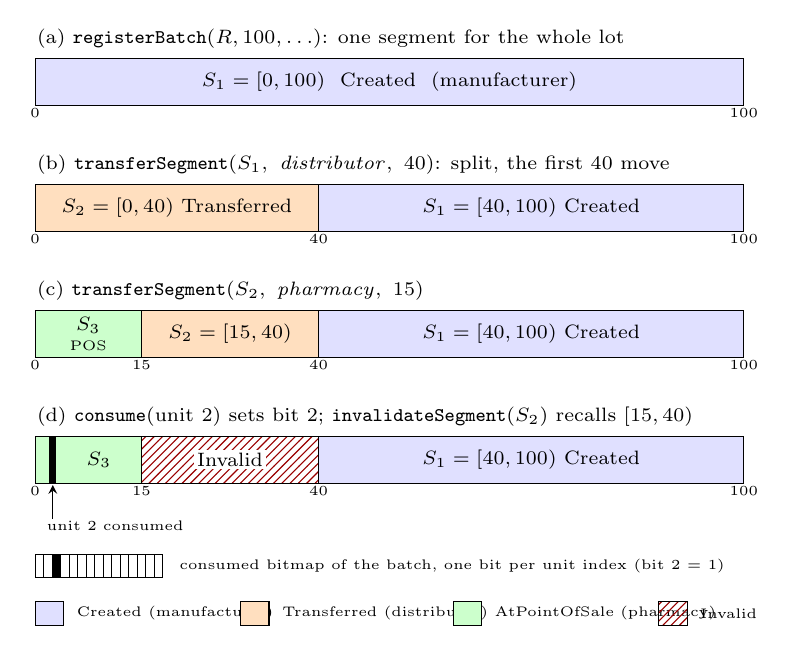
\begin{tikzpicture}[
  x=0.9mm, y=1mm,
  created/.style={draw, fill=blue!12},
  transferred/.style={draw, fill=orange!25},
  atpos/.style={draw, fill=green!20},
  invalid/.style={draw, pattern=north east lines, pattern color=red!60!black},
  seg/.style={font=\scriptsize, inner sep=0.5pt, align=center},
  op/.style={font=\scriptsize, anchor=south west, inner sep=0.5pt},
  tick/.style={font=\tiny, anchor=north, inner sep=1pt},
]
  \def\h{6}
  % row: y offset, operation text, then segments
  \newcommand{\segbar}[4]{% #1 y, #2 start, #3 end, #4 style
    \path[#4] (#2,#1) rectangle (#3,#1+\h);}
  \newcommand{\ticks}[2]{% #1 y, #2 list
    \foreach \t in {#2} \node[tick] at (\t,#1) {\t};}

  % (a) registration
  \node[op] at (0,7) {(a) \texttt{registerBatch}$(R,100,\dots)$: one segment for the whole lot};
  \segbar{0}{0}{100}{created}
  \node[seg] at (50,3) {$S_1=[0,100)$ \ Created \ (manufacturer)};
  \ticks{0}{0,100}

  % (b) manufacturer -> distributor
  \node[op] at (0,-9) {(b) \texttt{transferSegment}$(S_1,\ \mathit{distributor},\ 40)$: split, the first 40 move};
  \segbar{-16}{0}{40}{transferred}
  \segbar{-16}{40}{100}{created}
  \node[seg] at (20,-13) {$S_2=[0,40)$ Transferred};
  \node[seg] at (70,-13) {$S_1=[40,100)$ Created};
  \ticks{-16}{0,40,100}

  % (c) distributor -> pharmacy
  \node[op] at (0,-25) {(c) \texttt{transferSegment}$(S_2,\ \mathit{pharmacy},\ 15)$};
  \segbar{-32}{0}{15}{atpos}
  \segbar{-32}{15}{40}{transferred}
  \segbar{-32}{40}{100}{created}
  \node[seg] at (7.5,-29) {$S_3$\\[-1pt]{\tiny POS}};
  \node[seg] at (27.5,-29) {$S_2=[15,40)$};
  \node[seg] at (70,-29) {$S_1=[40,100)$ Created};
  \ticks{-32}{0,15,40,100}

  % (d) consume of unit 2, recall of S2
  \node[op] at (0,-41) {(d) \texttt{consume}(unit 2) sets bit 2; \texttt{invalidateSegment}$(S_2)$ recalls $[15,40)$};
  \segbar{-48}{0}{15}{atpos}
  \segbar{-48}{15}{40}{invalid}
  \segbar{-48}{40}{100}{created}
  \fill[black] (2,-48) rectangle (3,-48+\h);
  \node[seg] at (9,-45) {$S_3$};
  \node[seg, fill=white, inner sep=1pt] at (27.5,-45) {Invalid};
  \node[seg] at (70,-45) {$S_1=[40,100)$ Created};
  \ticks{-48}{0,15,40,100}
  \draw[<-, >=stealth] (2.5,-48.2) -- ++(0,-4.3) node[anchor=north west, xshift=-1mm, font=\tiny, inner sep=0.5pt] {unit 2 consumed};

  % bitmap strip for the consumed set
  \begin{scope}[shift={(0,-60)}]
    \foreach \i in {0,...,14} \draw[fill=white] (\i*1.2,0) rectangle ++(1.2,3);
    \fill[black] (2*1.2,0) rectangle ++(1.2,3);
    \node[font=\tiny, anchor=west] at (19,1.5) {consumed bitmap of the batch, one bit per unit index (bit 2 = 1)};
  \end{scope}

  % legend
  \begin{scope}[shift={(0,-66)}]
    \path[created] (0,0) rectangle ++(4,3);      \node[font=\tiny, anchor=west] at (4.5,1.5) {Created (manufacturer)};
    \path[transferred] (29,0) rectangle ++(4,3); \node[font=\tiny, anchor=west] at (33.5,1.5) {Transferred (distributor)};
    \path[atpos] (59,0) rectangle ++(4,3);       \node[font=\tiny, anchor=west] at (63.5,1.5) {AtPointOfSale (pharmacy)};
    \path[invalid] (88,0) rectangle ++(4,3);     \node[font=\tiny, anchor=west] at (92.5,1.5) {Invalid};
  \end{scope}
\end{tikzpicture}
\end{document}
